\documentclass[12pt,a4paper]{article}

% IMPORTACIÓN PAQUETES
% Acentos
\usepackage[utf8]{inputenc}
\usepackage[T1]{fontenc}
% Idioma español
\usepackage[spanish]{babel}
% Insertar imágenes
\usepackage{graphicx}
% Subfiguras
\usepackage{subcaption}
% Espaciado
\usepackage{setspace}
% Comillas inteligentes
\usepackage{csquotes}
% Márgenes
\usepackage{geometry}
\geometry{margin=2.5cm}
% Hipervínculos
\usepackage{hyperref}
\hypersetup{
    colorlinks=true,
    linkcolor=black,
    citecolor=black,
    urlcolor=black
}
% Referencias inteligentes
\usepackage{cleveref}

% Configuración de cleveref en español
\crefname{figure}{figura}{figuras}
\Crefname{figure}{Figura}{Figuras}
\crefname{subfigure}{figura}{figuras}
\Crefname{subfigure}{Figura}{Figuras}
\crefname{enumi}{pregunta}{preguntas}
\Crefname{enumi}{Pregunta}{Preguntas}

% Conjunciones en español
\AtBeginDocument{\renewcommand{\creflastconjunction}{ y~}}
\AtBeginDocument{\renewcommand{\crefrangeconjunction}{ a~}}
\AtBeginDocument{\renewcommand{\crefmiddleconjunction}{, }}

% Para no repetir la carpeta de resultados en cada imagen
\graphicspath{{resultados/}}

% Título y autoría
\title{\textbf{Impresiones sobre la IA en mi familia}}
\author{Haessler Joan Ortiz Moncada \\[0.5cm]
        Universidad Distrital Francisco José de Caldas \\
        Facultad de Ingeniería \\
        Curso: BIG DATA}
\date{\today}

\begin{document}

% Título
\maketitle

% Introducción
\section*{Introducción}
La Inteligencia Artificial (IA) es hoy en día un término que parece estar de moda: lo escuchamos en los noticieros, 
aparece en comentarios de diferentes contenidos en redes sociales y se aborda en el ámbito académico, 
desde los colegios hasta las universidades. Sin embargo, al conversar con varios miembros de mi familia, noté que el 
concepto de IA no está claramente definido, se comprende de diferentes maneras y tampoco existe claridad sobre su alcance.

Con la intención de recopilar las impresiones, ideas y prejuicios que mi familia tiene sobre la IA, diseñé una breve 
encuesta que me permitiera recoger estos pensamientos. De esta forma, busco hacerme una idea de cómo mi familia, 
a la que considero representativa de muchas familias colombianas, percibe e interpreta el término IA.

% Desarrollo
\section*{Desarrollo}
Las preguntas que realicé a mi familia mediante un formulario de Google fueron las siguientes:

\begin{enumerate}
    \item ¿En qué grupo etario se encuentra? \label{it:p1}
    \begin{itemize}
        \item Menos de 15 años
        \item 15 a 25 años
        \item 26 a 40 años
        \item 41 a 60 años
        \item Más de 60 años
    \end{itemize}
    \item ¿Cuál es el nivel educativo más alto que ha alcanzado? \label{it:p2}
    \begin{itemize}
        \item Primaria
        \item Bachillerato
        \item Técnico
        \item Profesional
        \item Posgrado
    \end{itemize}
    \item Del 1 al 5, ¿qué tan familiarizado está con el término "Inteligencia Artificial"? \label{it:p3}
    \item ¿Puede nombrar algunos ejemplos de IA que encuentre en su vida diaria? \label{it:p4}
    \begin{itemize}
        \item Sí
        \item No
    \end{itemize}
    \item Si la respuesta a la pregunta anterior fue "Sí", mencione algunos ejemplos de IA que 
    encuentre en su vida diaria. Separe los ejemplos con un guion (-). \label{it:p5}
    \item ¿Confía usted en los sistemas de inteligencia artificial (ej. conducción autónoma, servicio al cliente, bioseguridad)? \label{it:p6}
    \begin{itemize}
        \item Sí
        \item No
    \end{itemize}
    \item ¿Por qué confía o por qué no confía en los sistemas de inteligencia artificial? \label{it:p7}
    \item ¿Qué le preocupa sobre el desarrollo de la IA? \label{it:p8}
    \item ¿Qué tan cómodo se siente con que las empresas recopilen y utilicen sus datos personales? \label{it:p9}
    \item Dé ejemplos de situaciones de su vida diaria en las que grandes cantidades de datos puedan
     mejorar su calidad de vida. Separe los ejemplos con un guion (-). \label{it:p10}
    \item Con relación con la pregunta anterior, ¿cree que el gobierno o las empresas están utilizando 
    los datos eficazmente para mejorar estas áreas? \label{it:p11}
    \begin{itemize}
        \item Sí
        \item No
    \end{itemize}
\end{enumerate}

Antes de analizar y concluir a partir de las respuestas obtenidas en la encuesta, 
es importante caracterizar la población que la respondió. Para ello, son especialmente relevantes las \cref{it:p1,it:p2}. 
Las \cref{fig:f1,fig:f2} muestran esta información:

\begin{figure}[h!]
    \centering
    \begin{subfigure}{0.45\linewidth}
        \centering
        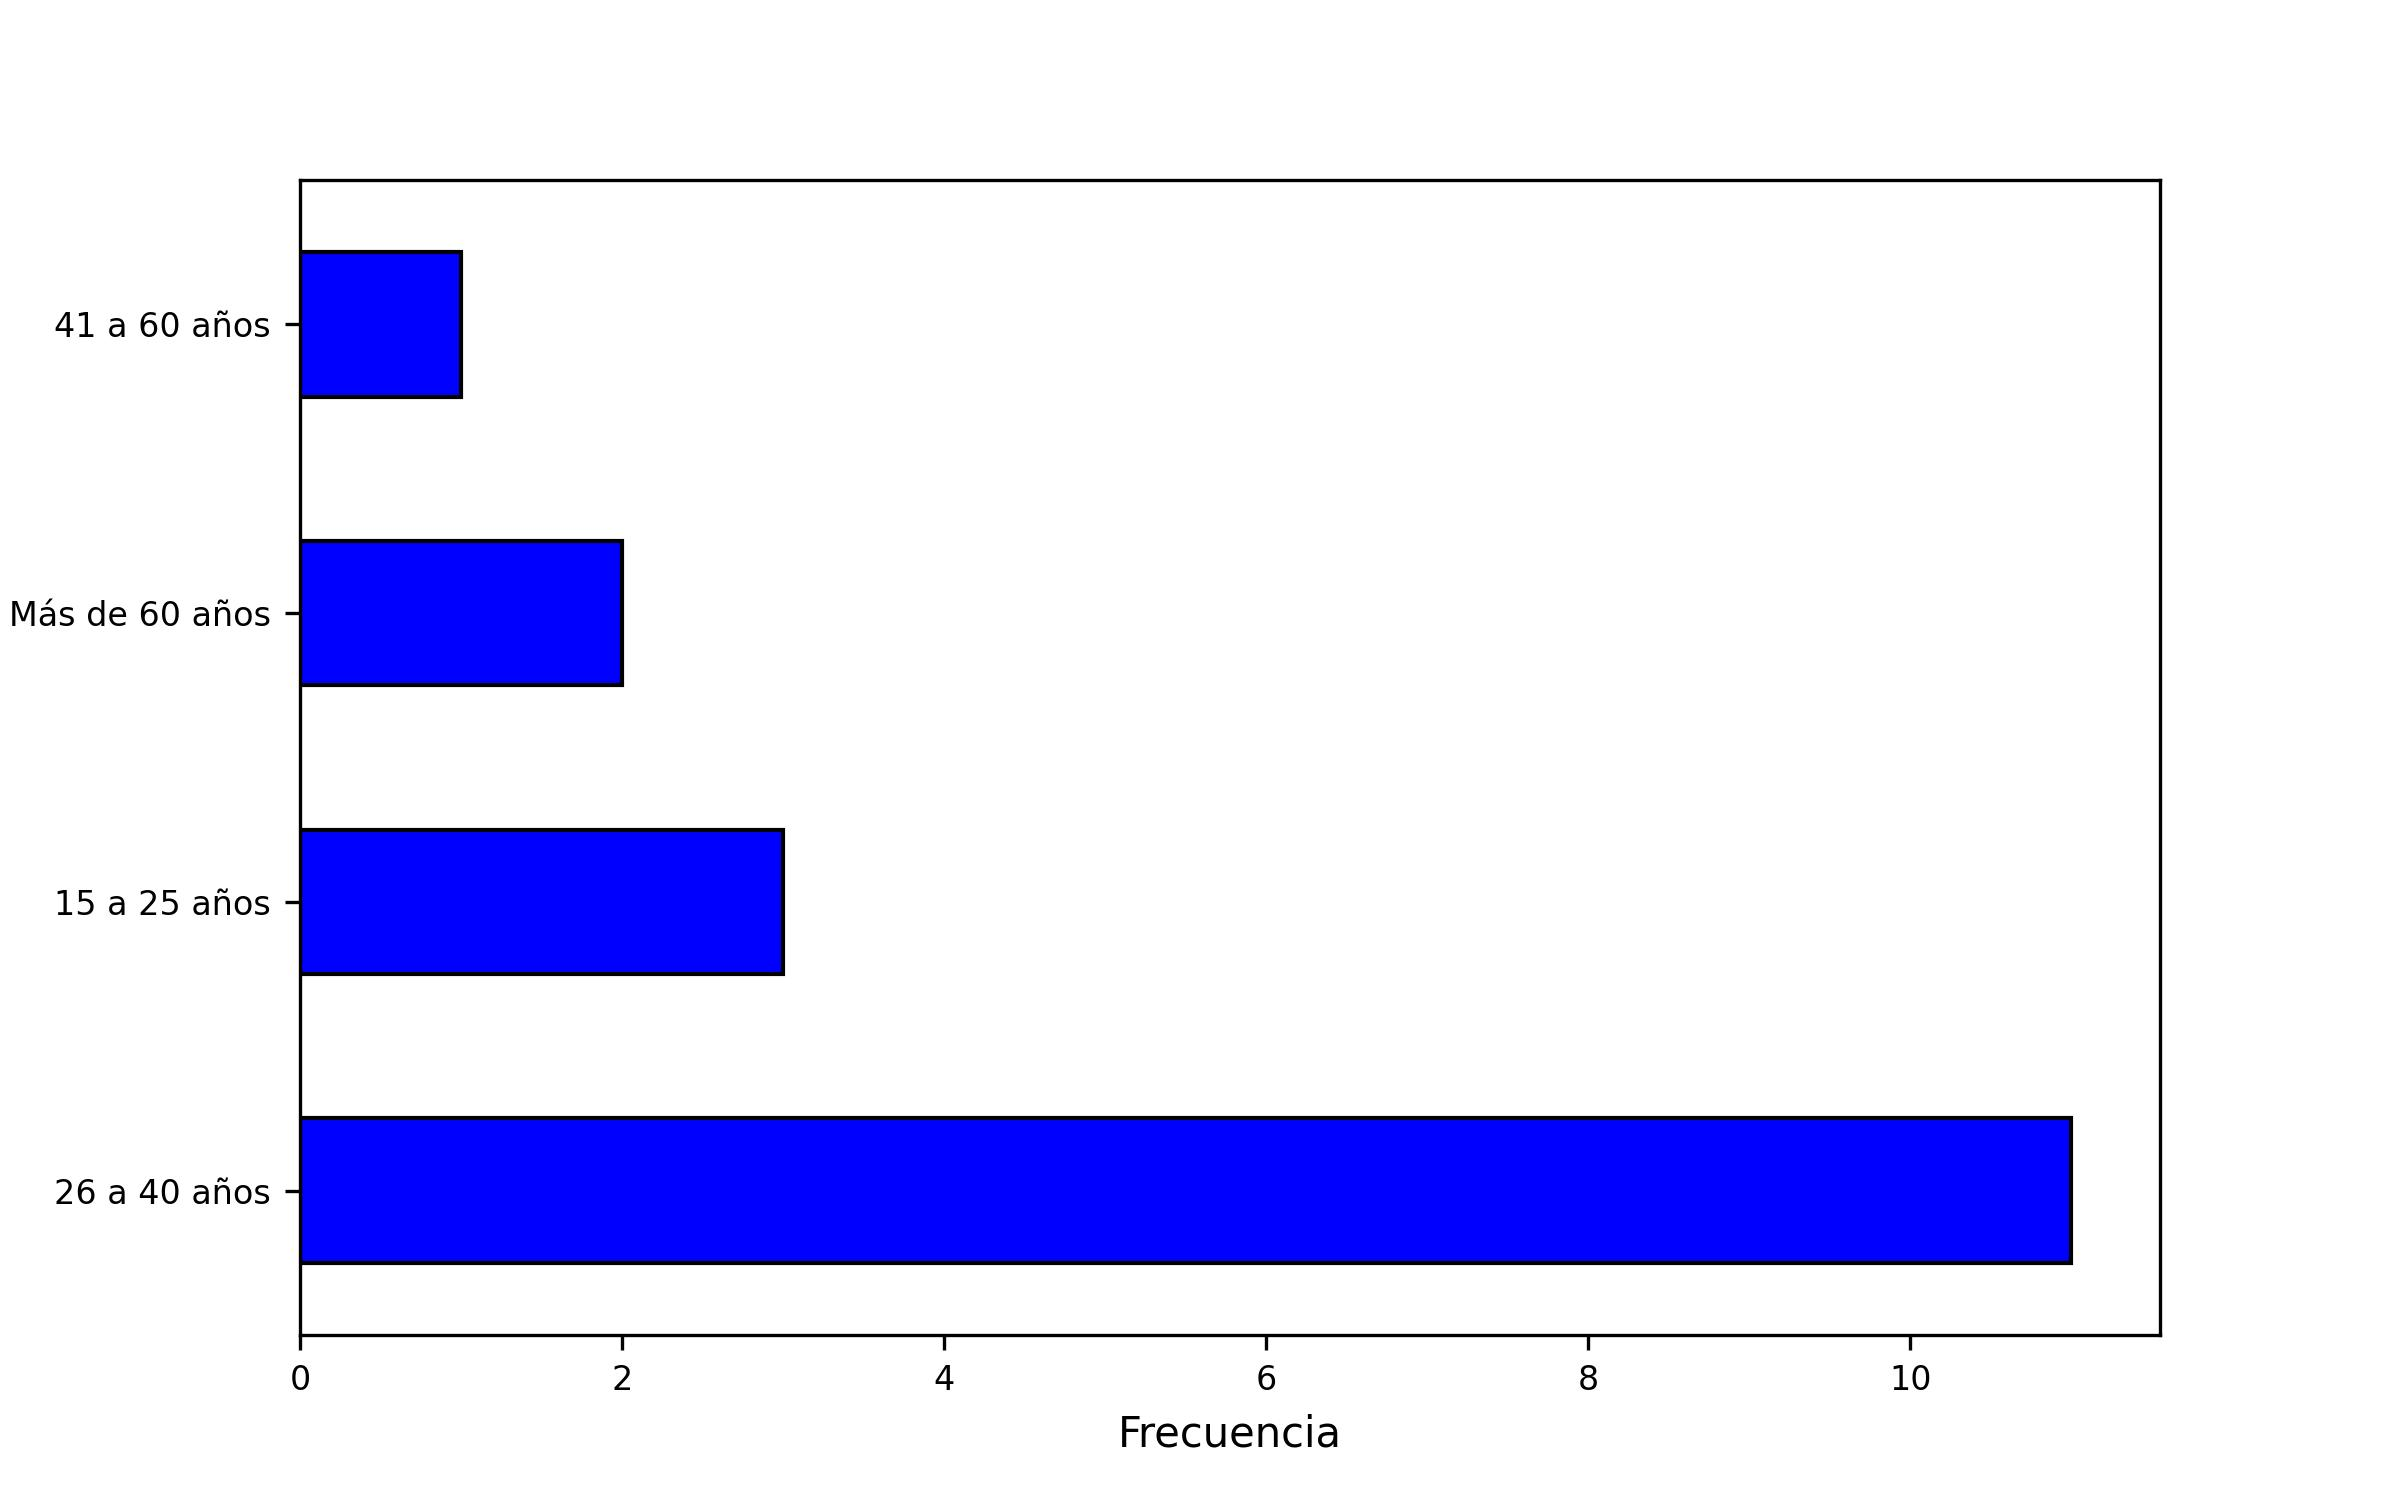
\includegraphics[width=\linewidth]{1_En que grupo etario se encuentra.jpg}
        \caption{Distribución por grupo etario}
        \label{fig:f1}
    \end{subfigure}
    \hfill
    \begin{subfigure}{0.45\linewidth}
        \centering
        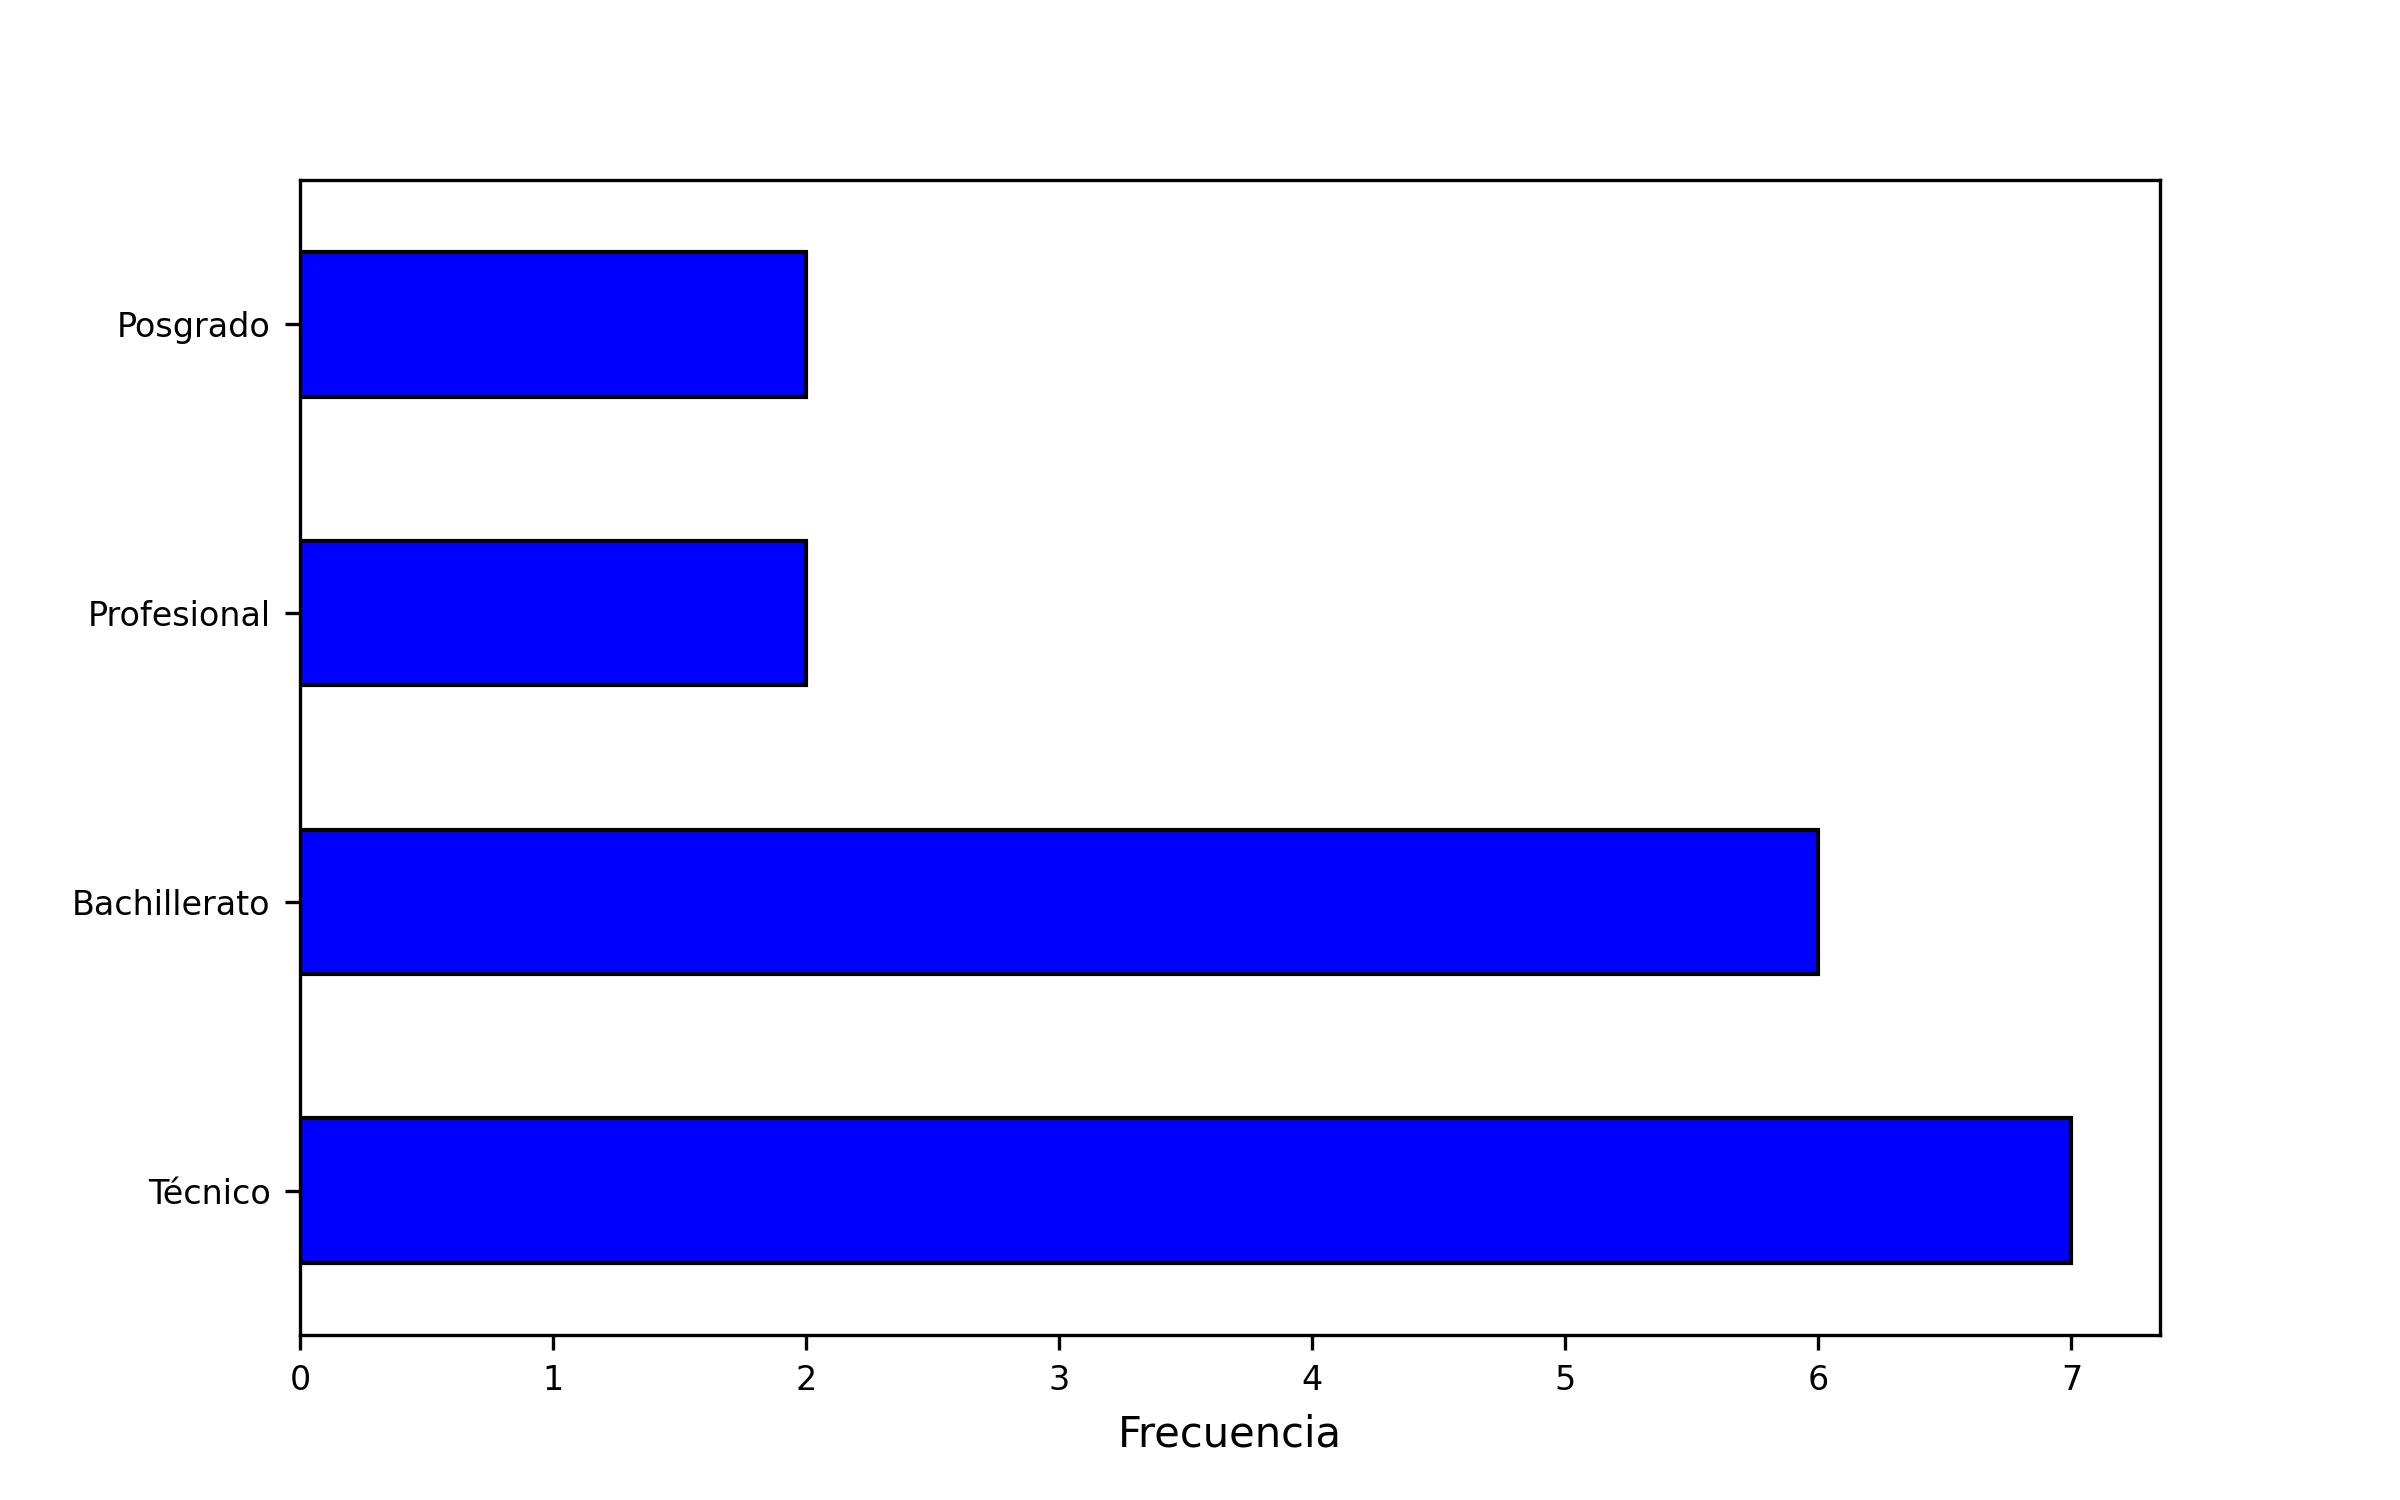
\includegraphics[width=\linewidth]{2_Cuál es el nivel educativo más alto que ha alcanzado.jpg}
        \caption{Nivel educativo más alto alcanzado}
        \label{fig:f2}
    \end{subfigure}
    \caption{Caracterización de la población encuestada}
\end{figure}

La mayoría de los encuestados se encuentra en el grupo etario de 26 a 40 años, y la mayoría de ellos 
ha alcanzado al menos un nivel educativo técnico. Esto permite concluir que la población presenta un sesgo, pues 
se trata de personas jóvenes, con un nivel educativo medio-alto, lo cual hace probable que tengan un 
mayor conocimiento sobre el término IA y sus aplicaciones.

Por otra parte, la \cref{it:p3} permite conocer la autopercepción que tienen los encuestados sobre su 
familiaridad con el término IA. Al calcular el promedio aritmético de las respuestas, 
se obtiene un valor de 3.76, lo que indica que la mayoría se siente medianamente familiarizada 
con el concepto de IA. 

Respecto a la \cref{it:p4}, la mayoría de los encuestados afirma que sí puede nombrar ejemplos de IA en 
su vida diaria. No obstante, al analizar las respuestas a la \cref{it:p5}, se observa que los ejemplos más 
comunes mencionados son ChatGPT, Copilot y Gémini, lo que indica que, en términos generales, existe una correcta asociación 
del concepto de IA con estos modelos de lenguaje populares. Sin embargo, también se mencionan aplicaciones como Indriver, 
Waze o incluso el almacenamiento en la nube, que no corresponden estrictamente a sistemas de IA. 

Por otra parte, las \cref{it:p6,it:p7} revelan que la mayoría de los encuestados no confía en los sistemas de IA. 
Las razones más frecuentes para esta desconfianza son la sensación de falta de privacidad, 
el temor de que el ser humano sea reemplazado por máquinas y la percepción de que los sistemas de IA pueden cometer errores graves en decisiones críticas, 
que deberían ser tomadas por humanos. 

Las \cref{fig:f3,fig:f4} ayudan a ilustrar esta información:

\begin{figure}[h!]
    \centering
    \begin{subfigure}{0.45\linewidth}
        \centering
        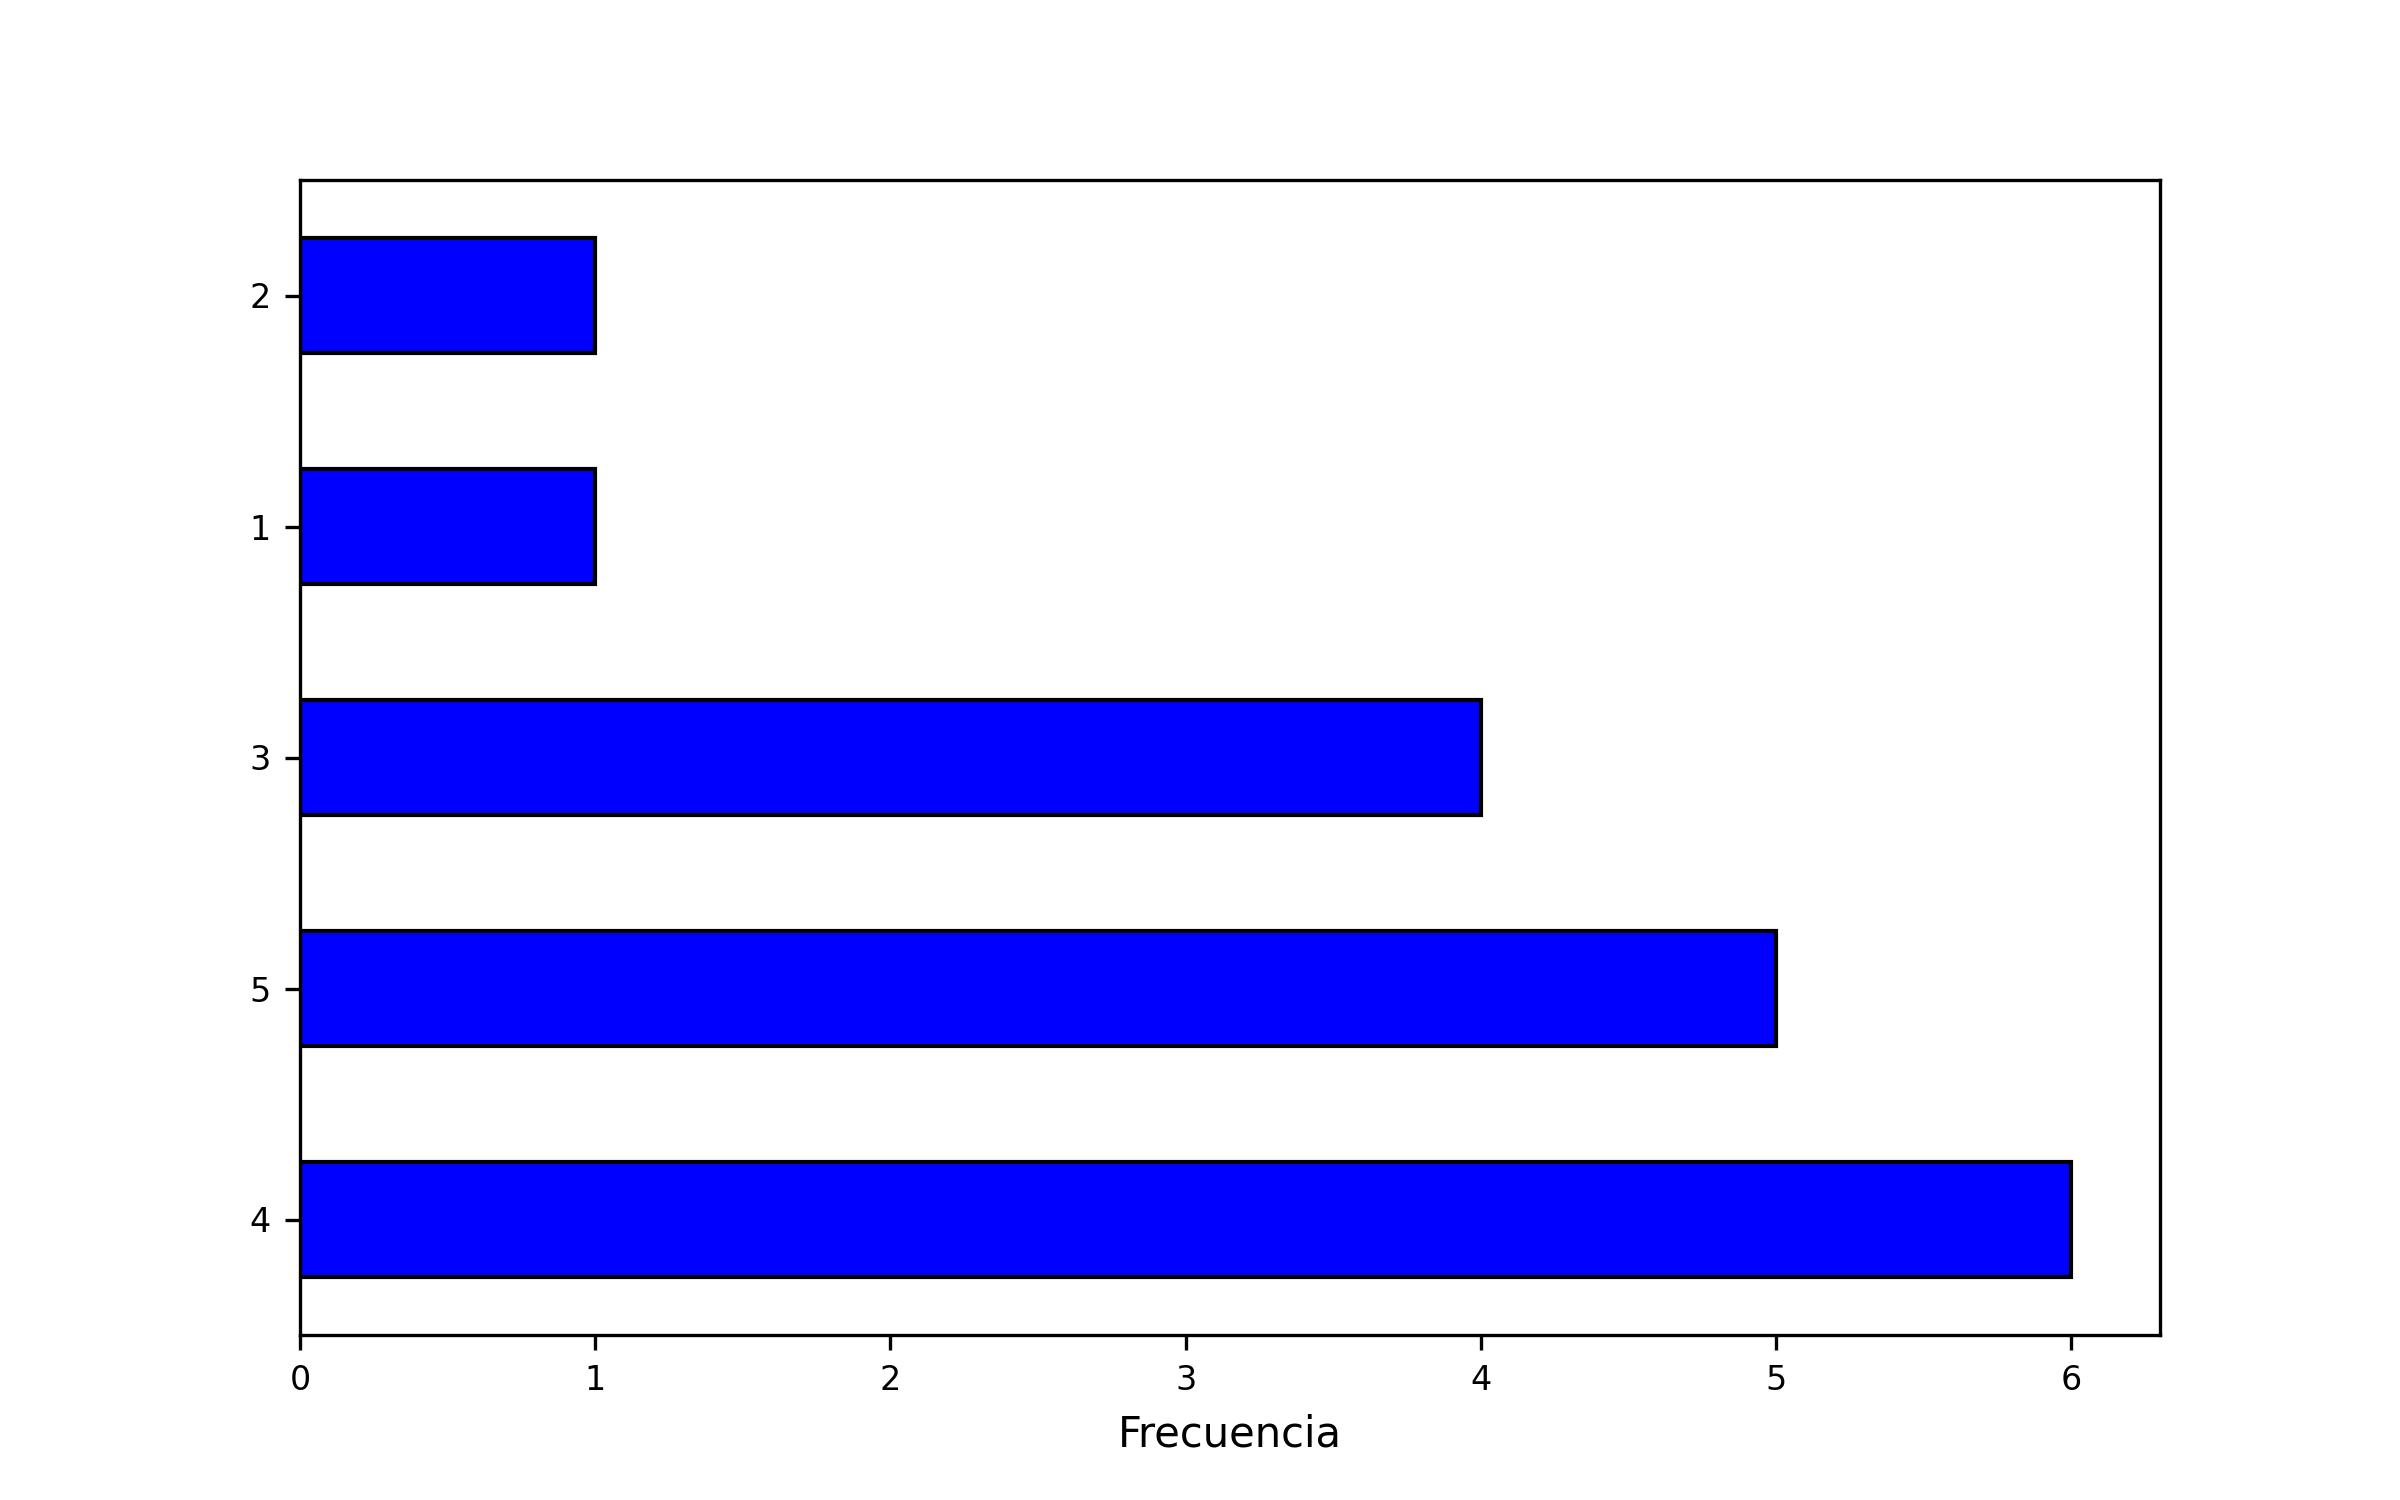
\includegraphics[width=\linewidth]{3_Del 1 al 5, Qué tan familiarizado está con el término Inteligencia Artificial.jpg}
        \caption{Nivel de familiaridad con el término IA}
        \label{fig:f3}
    \end{subfigure}
    \hfill
    \begin{subfigure}{0.45\linewidth}
        \centering
        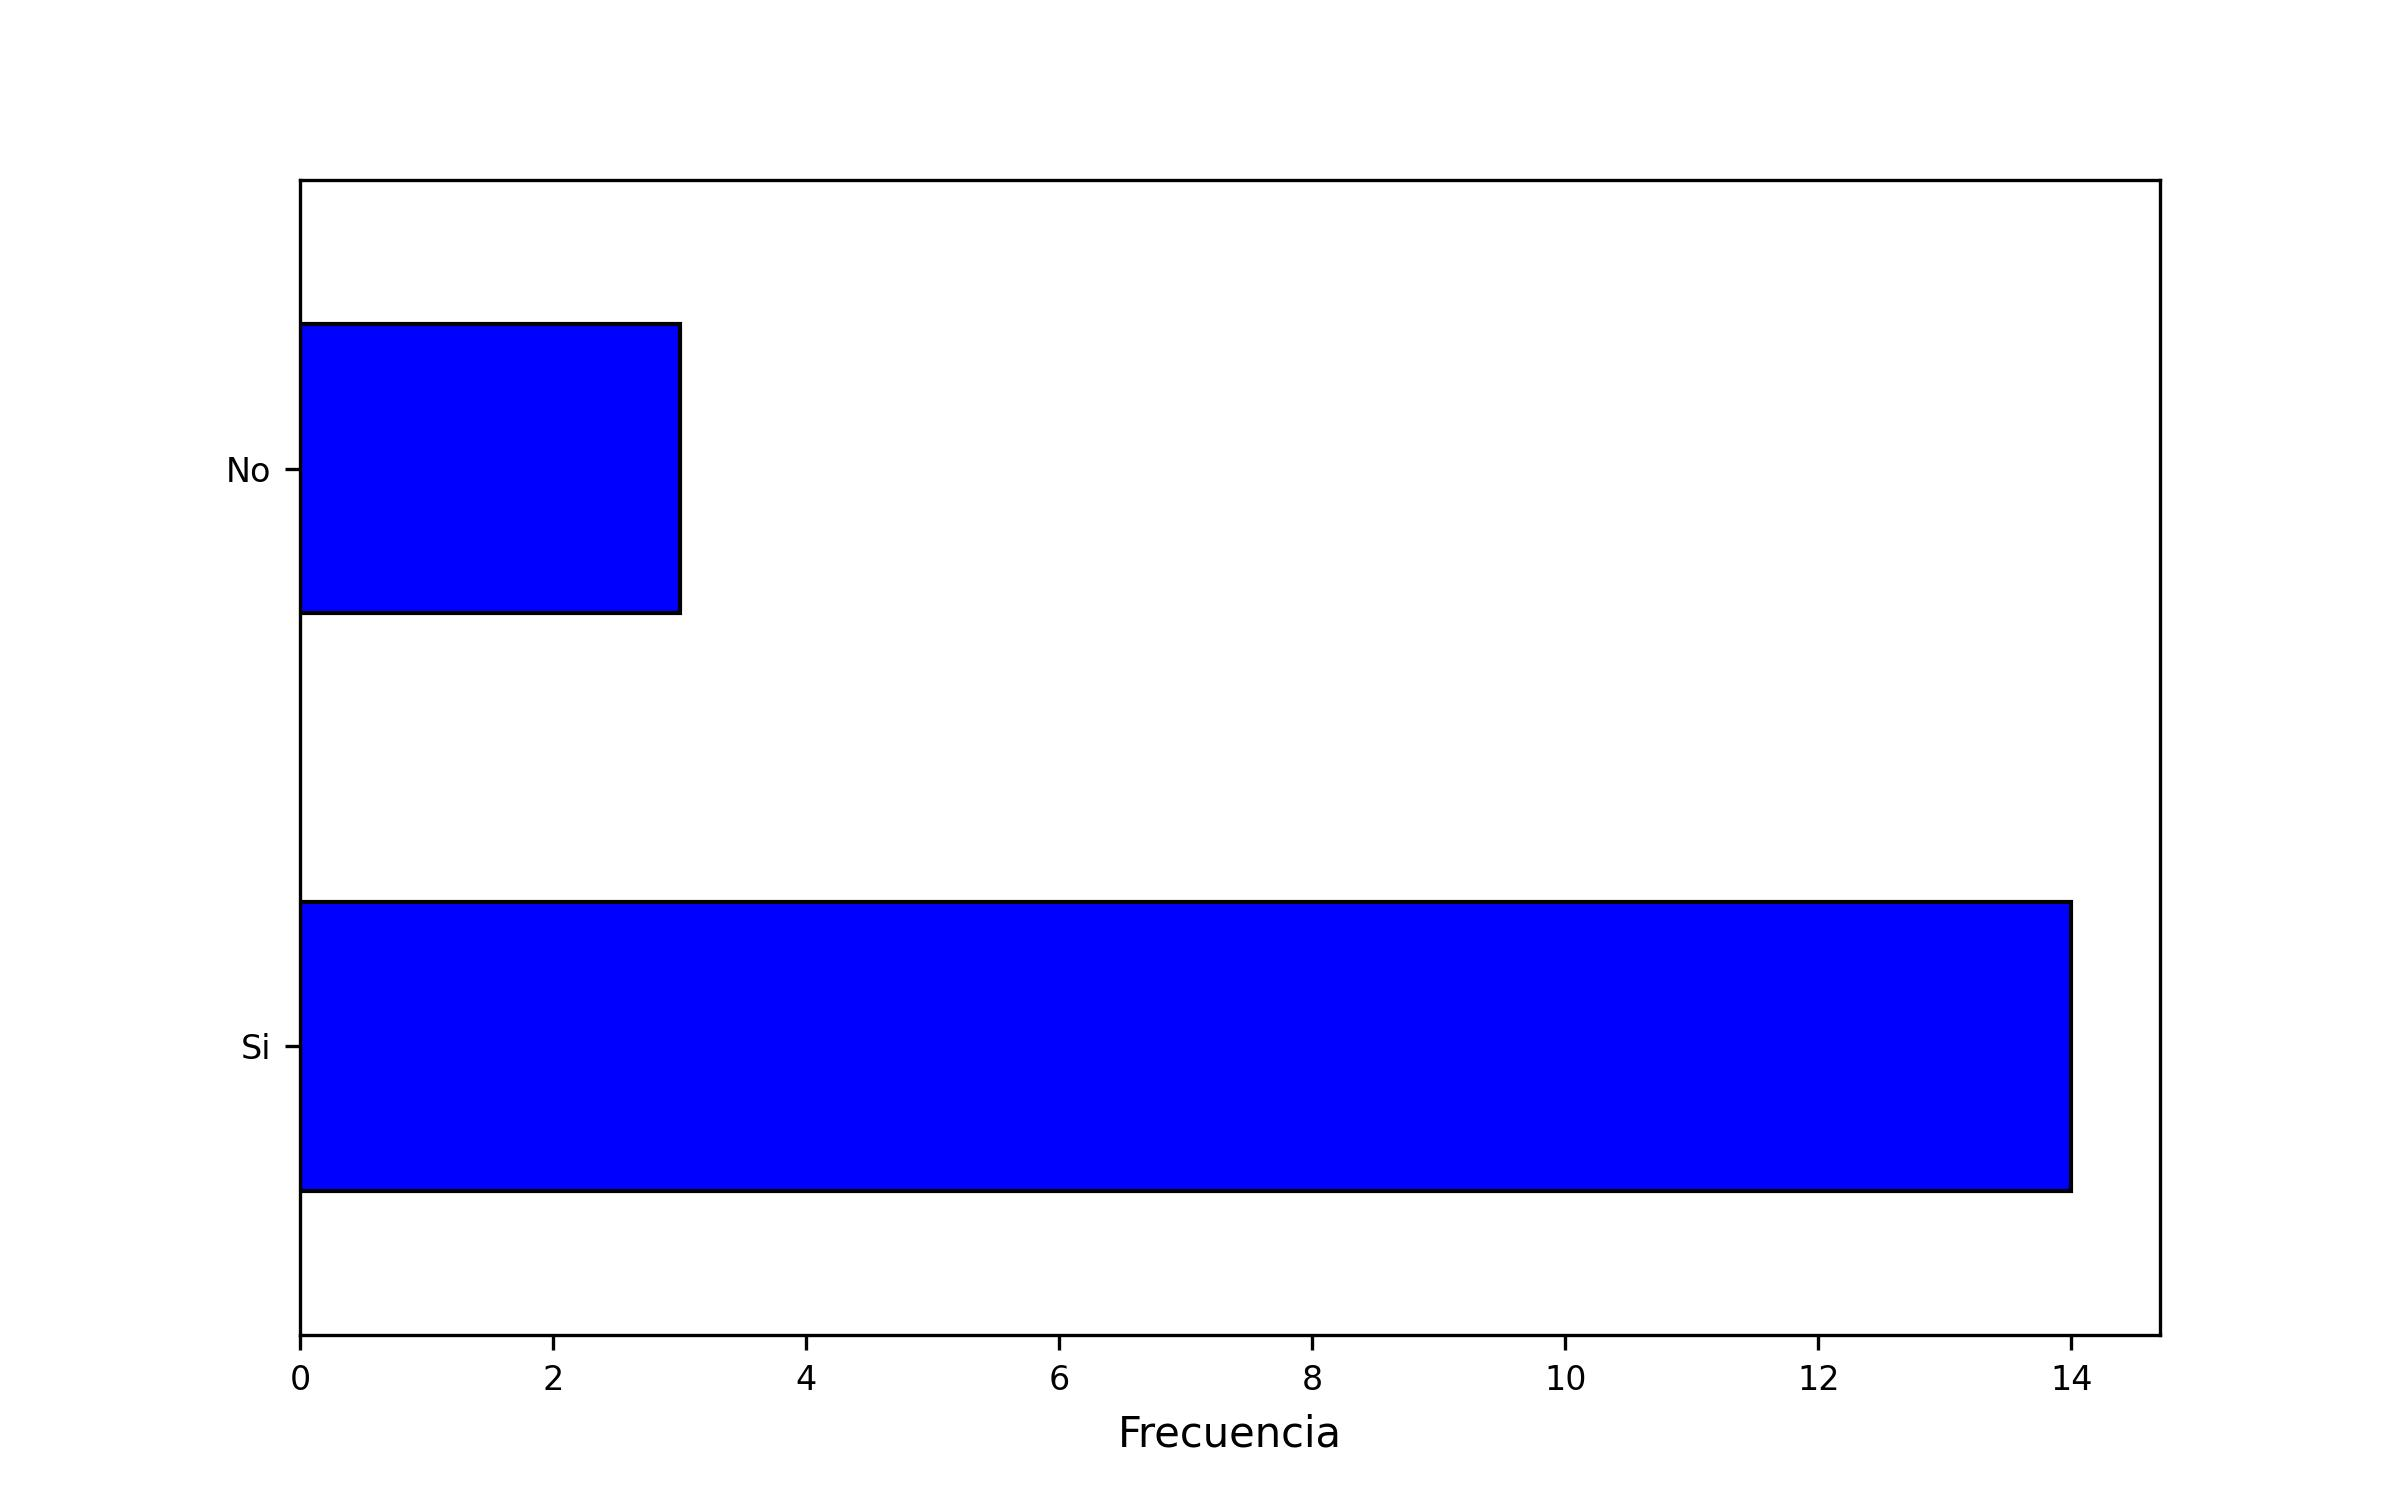
\includegraphics[width=\linewidth]{4_Puede nombrar algunos ejemplos de IA que encuentre en su vida diaria.jpg}
        \caption{Capacidad de dar ejemplos de IA}
        \label{fig:f4}
    \end{subfigure}
    \caption{Percepción de familiaridad y ejemplos de IA}
\end{figure}

\begin{figure}[h!]
    \centering
    \begin{subfigure}{0.45\linewidth}
        \centering
        \includegraphics[width=\linewidth]{5_Confía usted en los sistemas de inteligencia artificial.jpg}
        \caption{Confianza en los sistemas de IA}
        \label{fig:f5}
    \end{subfigure}
    \hfill
    \begin{subfigure}{0.45\linewidth}
        \centering
        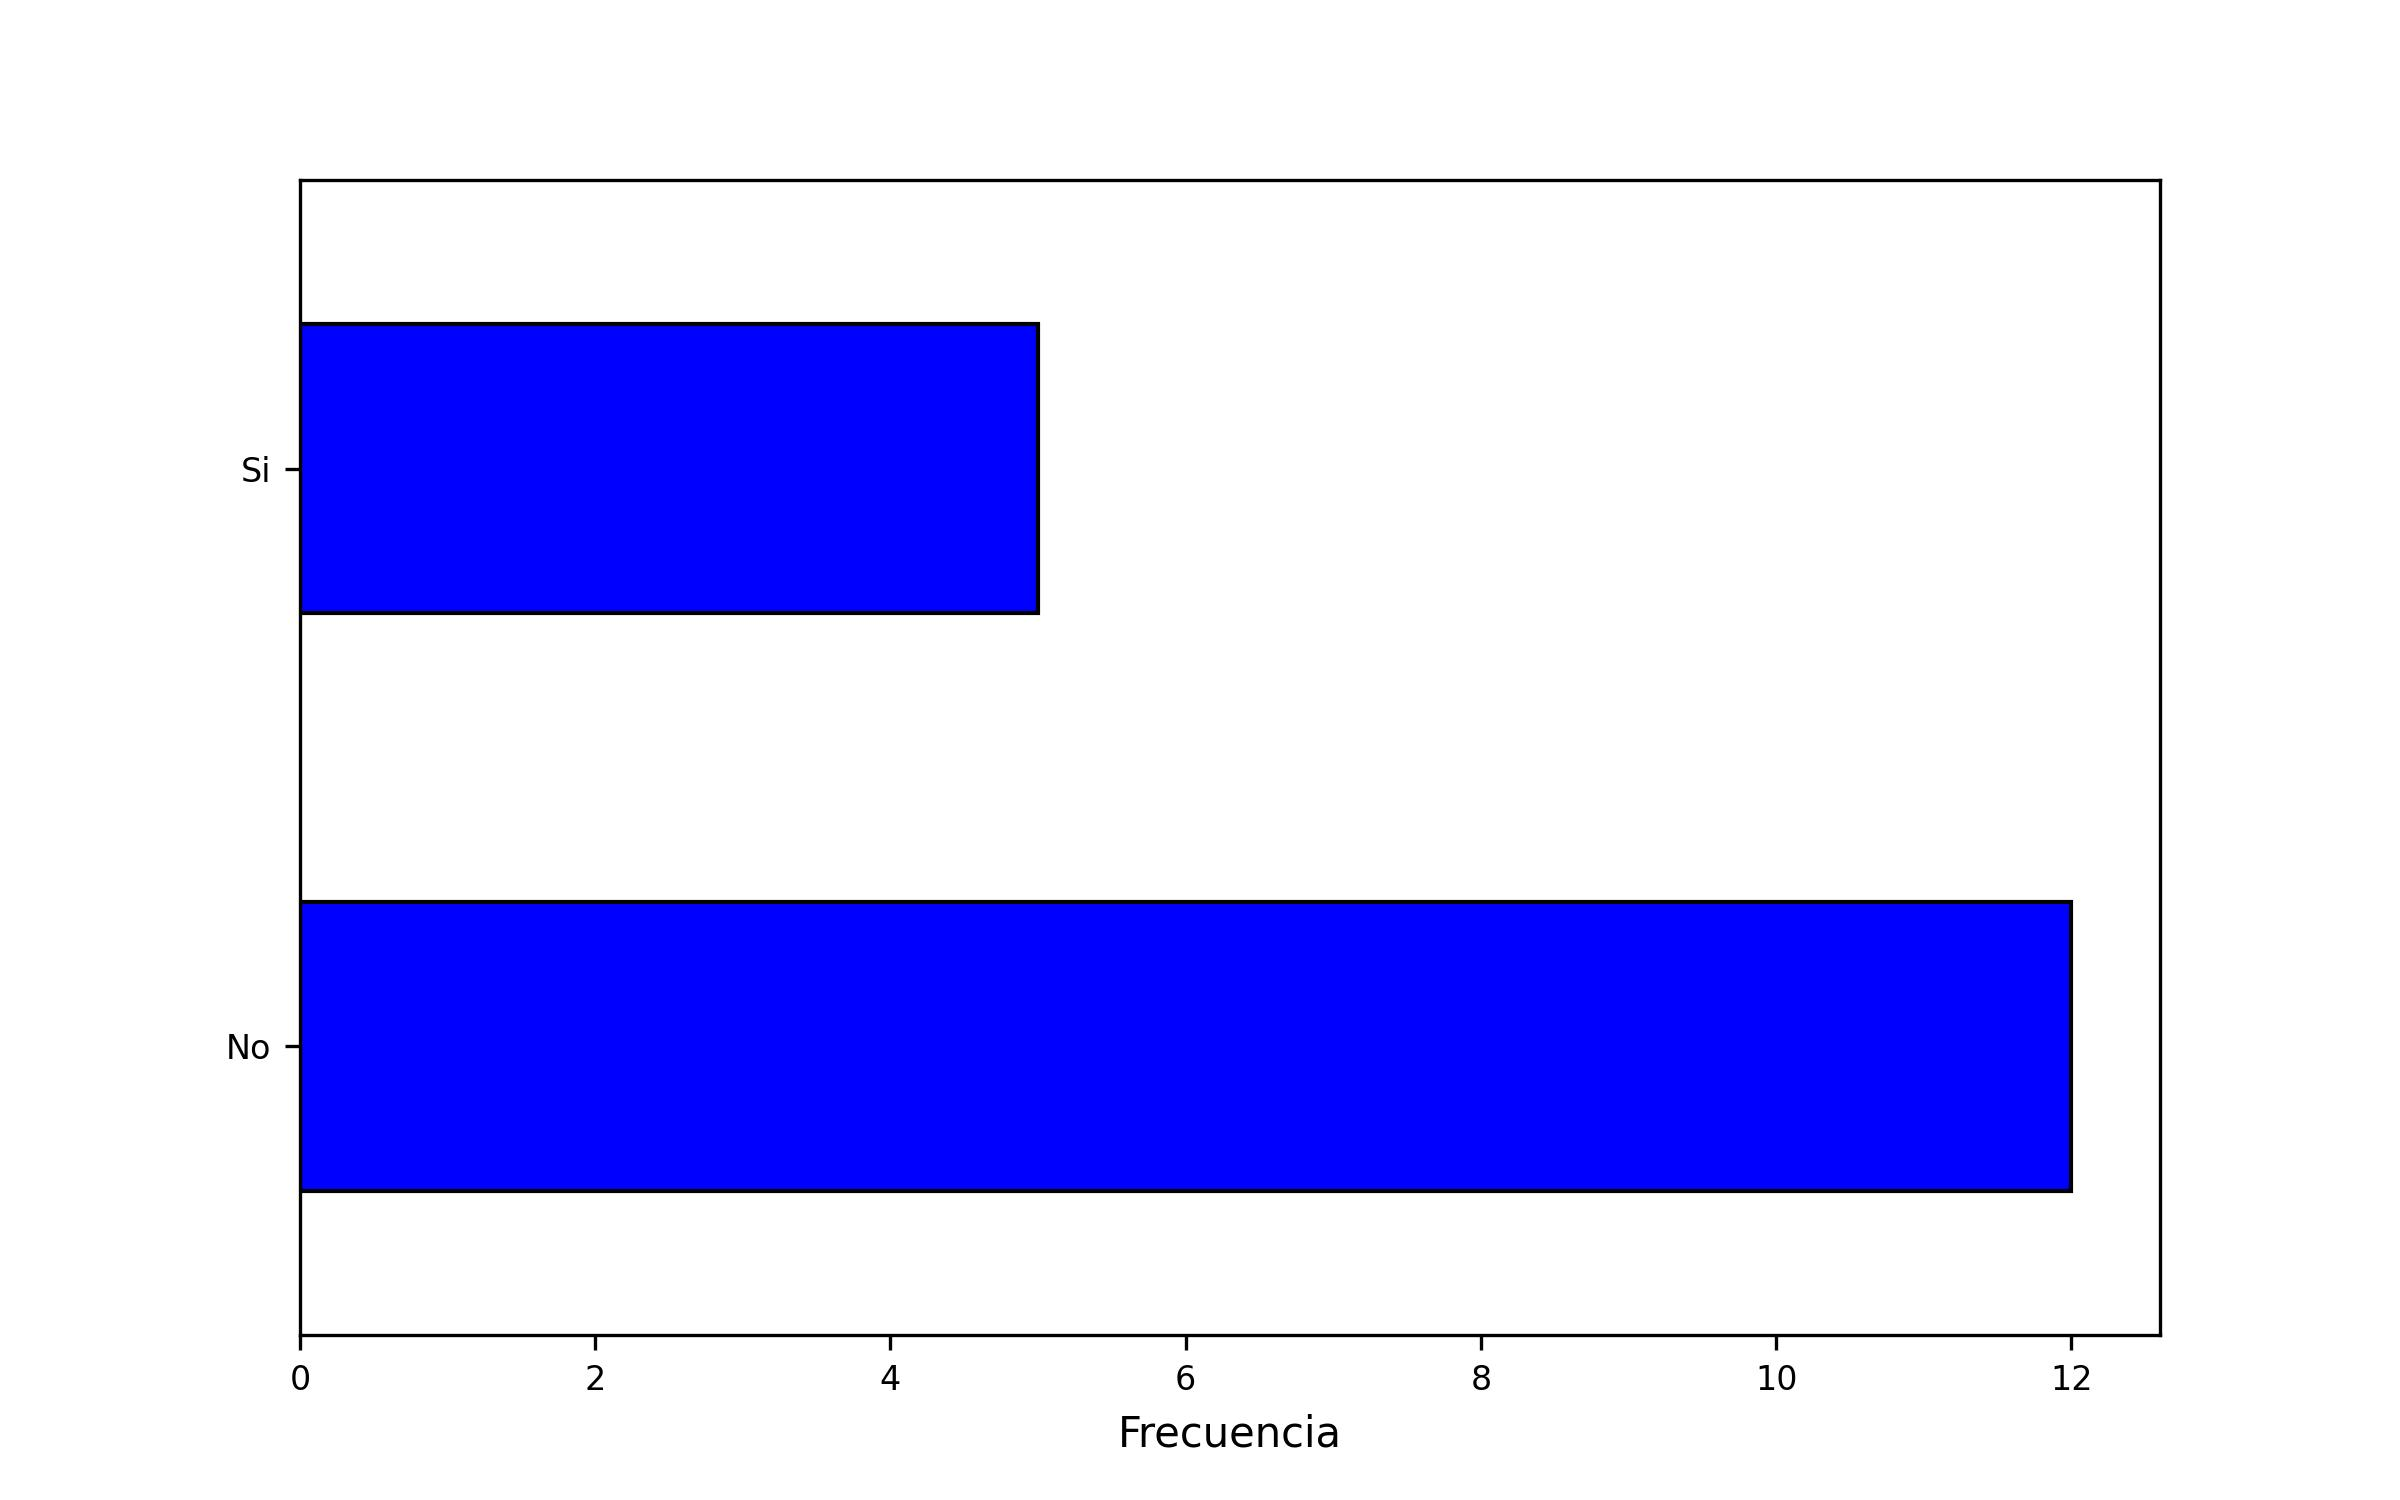
\includegraphics[width=\linewidth]{10_Cree que el gobierno o las empresas están utilizando los datos eficazmente para mejorar estas áreas.jpg}
        \caption{Percepción sobre el uso de datos por parte del gobierno y las empresas}
        \label{fig:f6}
    \end{subfigure}
    \caption{Confianza y percepción sobre uso de datos}
\end{figure}

% Conclusión
\section*{Conclusiones}
La encuesta realizada a mi familia permite obtener una visión general sobre cómo una familia colombiana
relativamente promedio percibe el término IA. A partir de esta encuesta, se puede concluir que la IA se entiende como 
una tecnología que permite a las máquinas realizar tareas de alta complejidad que normalmente requieren inteligencia humana,
y que además lo hacen en tiempo récord. 

No obstante, la percepción de su funcionamiento, alcance y aplicaciones es limitada; incluso parece difícil 
diferenciar qué es IA y qué no lo es, pues se mencionan aplicaciones que no la implementan realmente. 
Para varios miembros de mi familia, la IA es comparable a un buscador de Google o a un asistente virtual, 
lo que indica que la comprensión sobre esta tecnología es superficial y no se relaciona con sus capacidades más avanzadas.

Por otra parte, la encuesta evidencia una clara falta de confianza en los sistemas de IA. 
La mayoría considera que la IA debe ser únicamente una herramienta de apoyo para el ser humano, 
pero no un reemplazo. Asimismo, coinciden en que las decisiones críticas deben seguir siendo tomadas por personas. 
Esto refleja que, aunque varios encuestados utilizan sistemas de IA, sienten recelo por la posibilidad de que esta tecnología reemplace al ser humano 
en ciertas tareas, así como por la idea de que múltiples aspectos de la vida cotidiana podrían ser monitoreados y controlados por la IA.
\end{document}
